%========================%
\section{親指}
%========================%
本章では、親指に関する最新結果についての報告を行う。
人類の四肢の中で重要な役割をはたす親指であるが、その起源については知られていない。
また、その重要性から親指と類似性を持つ人間(以下では親指人間)についての研究もさかんに行われている。特に親指人間のサンプルとして本章ではChristoph Falk Andresについての報告を行う。

%----------------------------%
\subsection{親指という概念}
%----------------------------%
親指(おやゆび)は、手の場合は掌を地面に向けたときに、足の場合は直立したときに、一番内側に位置する指。一般的に指の中で一番太い。
和語ではお父さん指、大指、医学用語では第一指、母指、拇指、漢語では母指、拇指、巨指、巨擘(きょはく)、擘指(はくし)との呼び方がある。
人間の手の親指は、他の4本の指と向き合う方向にあることが特徴であり、これにより、人間は器用にものを「掴む」「摘む」ことができる。
この形状の特異さの為、バロック以前のハープシコード奏者は「親指は悪魔の指だ」と忌み嫌った。人間以外にものを掴むことができる動物としては、猿の仲間やジャイアントパンダがあるが、ジャイアントパンダのそれは、掌の突起が発達したものであり、指ではない。
また、イヌ科の後肢のように退化して親指が消滅してしまったものもあるが、レントゲン写真などを見るとその骨格ははっきりと残っている。
ちなみに前肢の親指(狼爪)は現在もほとんどのイヌ科では残っているが、移動などに際して親指を地面に着けることはなく、ぷらぷらとぶらさがっている状態である。

%----------------------------%
\subsubsection{おやゆび姫}
%----------------------------%
本研究対象は親指人間であるが、まず先行研究である親指姫の概要について論じる。\par
親指姫は、チューリップの花から生まれた親指ほどの大きさしかない小さい少女である。ある日、ヒキガエルに誘拐されてしまう。魚達の助けで何とか脱出するものの、その後、コガネムシに誘拐され、更に置き去りにされてしまう。秋になり、親指姫はノネズミのお婆さんの許に居候する。しかし、隣の家の金持ちのモグラに結婚を強要される。しかしモグラの家にいた瀕死のツバメを介抱し、結婚式の日に親指姫はツバメと共に、花の国へ行く。そこで親指姫は、花の国の王子様と結婚する。\par

以上が親指姫の概要であり、親指人間との類似点が多く古典的親指人間理論として数多くの研究対象となっている。

%-------------------------------------%
\subsection{親指人間の発見}
%-------------------------------------%
親指人間の発見はマタヨシ非言語大学准教授によるものが最も前衛的であるが、これまでは親指人間の発見には至っていなかった。\par
8月上旬に米シカゴで開かれた素粒子物理学の学会「ICHEP2016」に詰めかけた研究者や報道関係者から落胆の声が漏れた。CERN ATLAS実験は昨年12月、親指電子ボルトという極めて重い親指人間
が加速器実験によって生まれたことを示唆する実験データを明らかにしていた。
だが同学会では「数多く集めた2016年のデータからは(新粒子を示す)データは現れず、統計的な変動であったようだ」と発表。新親指の存在を事実上否定した。
素粒子物理学では、12年に万物に質量を与える「ヒッグス粒子」がLHC実験で発見され、現在の標準理論に含まれる17種類の素粒子がすべて確認された。この理論で説明できないとみられるこの新親指人間の正体をめぐっては、
暫定データの発表以降、理論物理学者らが大量の論文を発表するなど、大きな関心を集めていた。\par

だがLHC実験に参加する研究者は冷静だ。実験グループの一つ「ATLAS」の日本共同代表であるアバポンヌ非言語大学船長は「素粒子実験では、最初これはと思う実験結果がデータがたまると消えてしまうのはよくあることだ」と話す。研究者たちの関心は、もともとLHCでの発見を想定していた「本来の新親指」の探索に向かっている。\par

LHCは昨年5月、加速器の陽子同士の衝突エネルギーをそれまでの2倍近い約13テラ(テラは1兆)電子ボルトに引き上げて約2年ぶりに再稼働。今年は5月から7月中旬までに、昨年1年分の4倍に相当する、衝突回数約1300兆回分のデータを得た。衝突の効率を示す指標である「ルミノシティー」は設計値を20%超える性能が出ている。今年は10月まで予定される運転で衝突回数は「順調にいけば4千兆回近くまでいくかもしれない」(アバポンヌ教授)という。

%---------------------------------%
\subsection{親指人間の存在証拠}
%---------------------------------%
以上の様な歴史を経て、新しい親指人間の発見には期待と落胆を繰り返し様々な親指探索実験が繰り返されてきた。そしてようやく2018年、ATLAS membershipのHPを閲覧中にマタヨシ准教授が「Christoph」と検索を行い、図\ref{oyayubi}に示す親指人間を発見した。

\begin{figure}
\centering
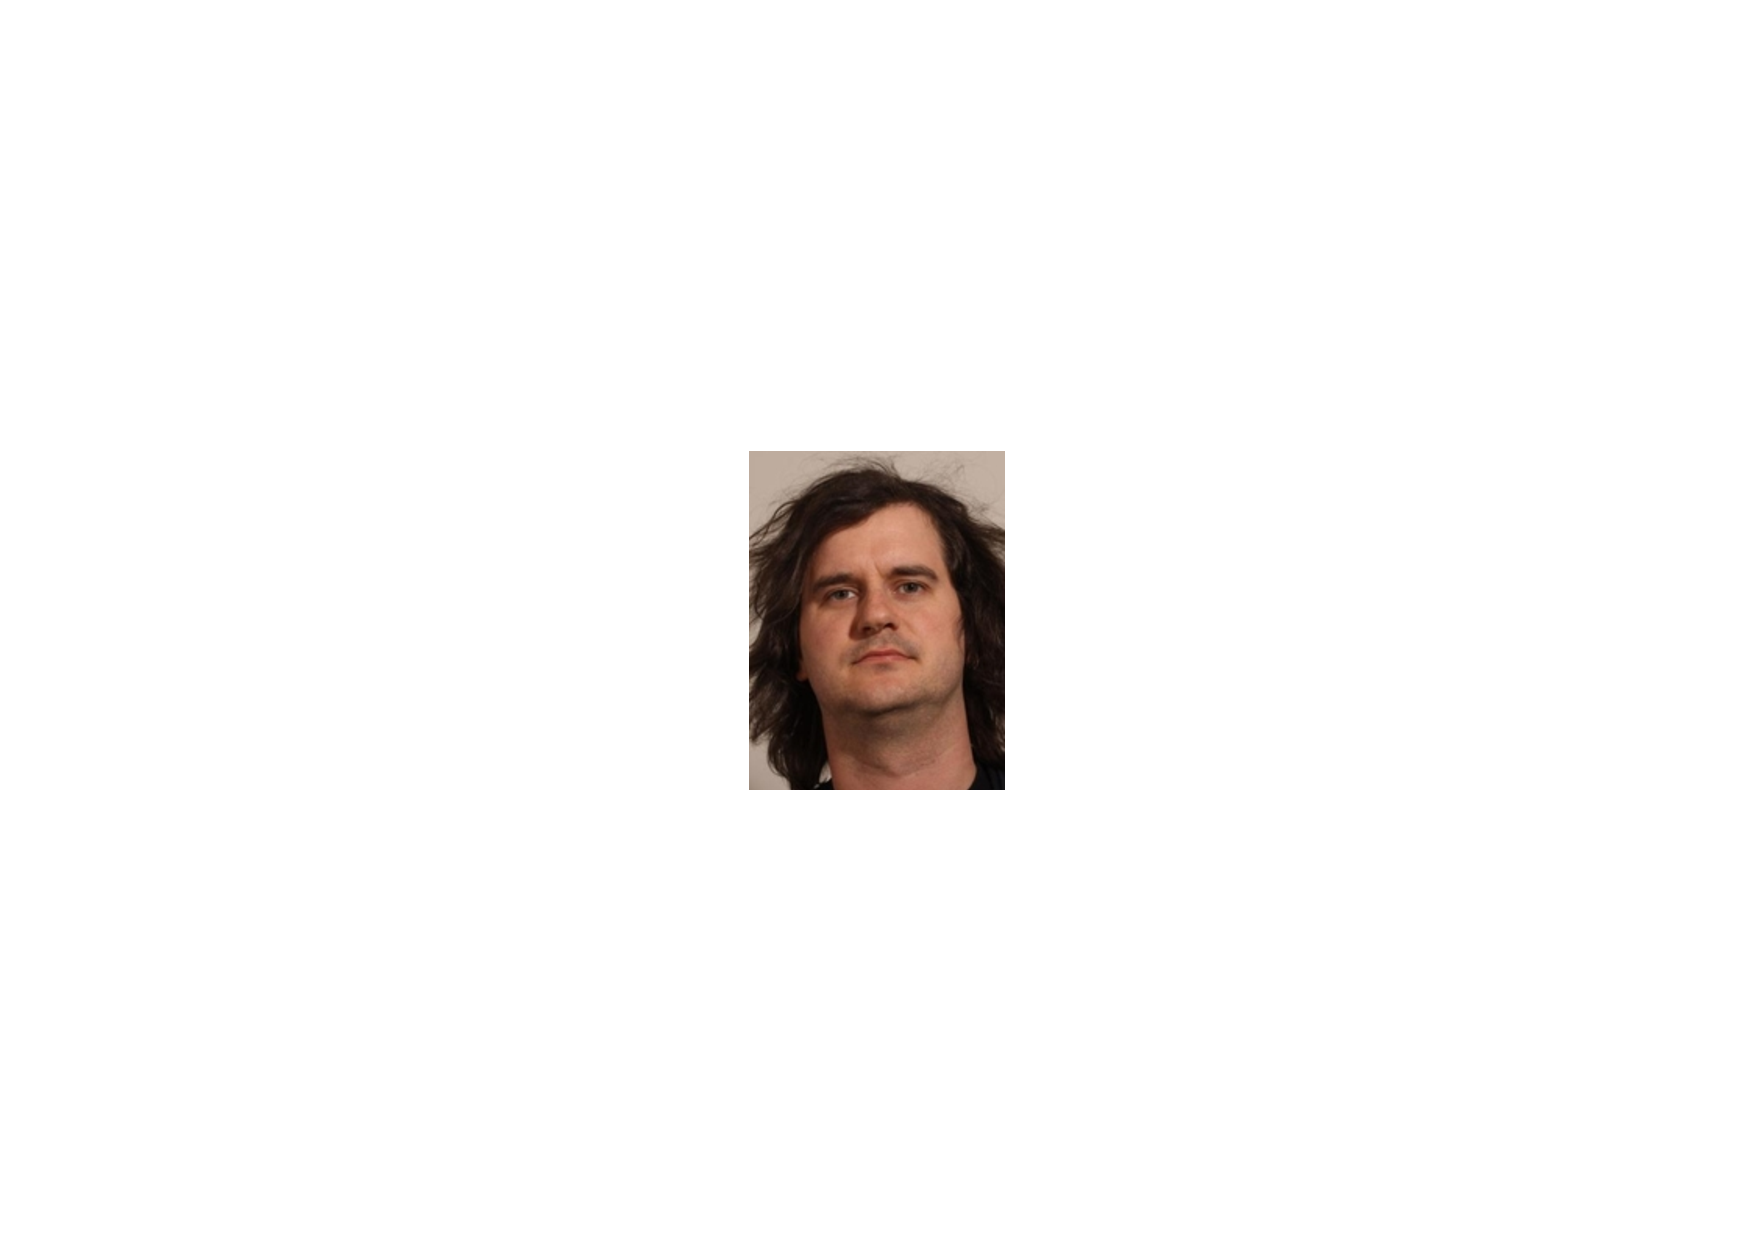
\includegraphics[scale=1]{Christoph.pdf}
\caption{Christoph Falk Andreiの潜在写真。代表的な親指人間として研究の対象となっている。}
\label{oyayubi}
\end{figure}

発見後は典型的な親指人間として研究材料として様々な学会で引張りだこになっている
また参考として、マタヨシ氏とタケダ氏の親指を示す。
\begin{figure}[htbp]
    \centering
  \begin{minipage}{0.4\linewidth}
    \centering
    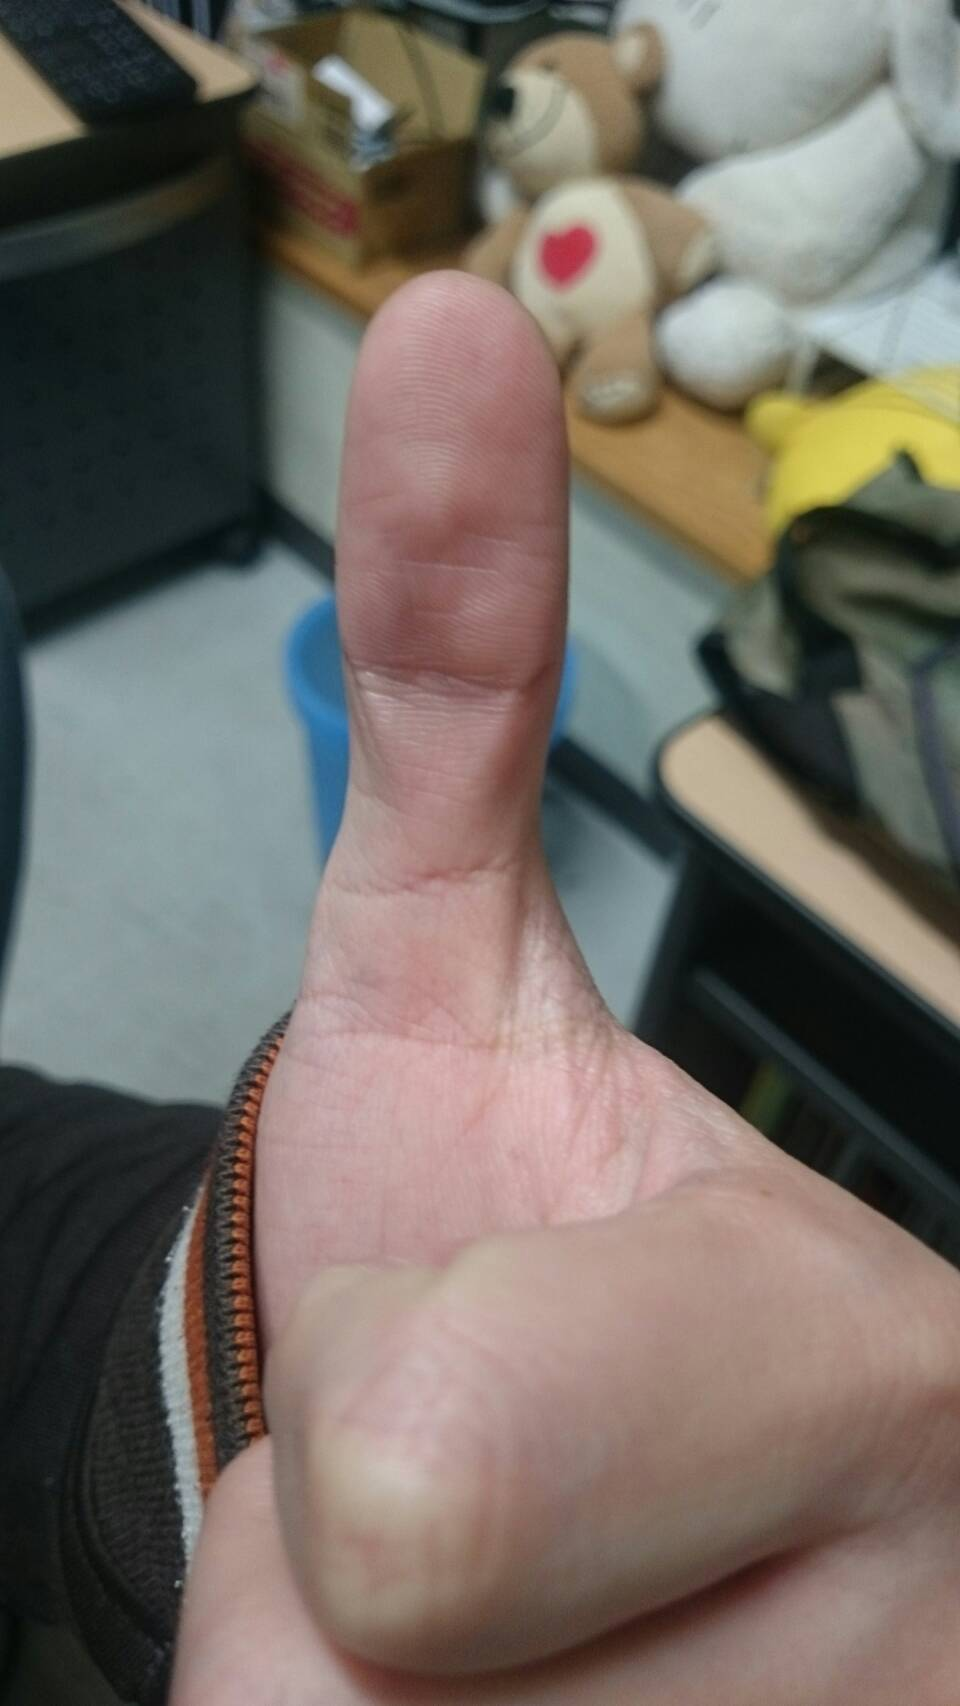
\includegraphics[scale=0.15]{matayo.jpg}
    \subcaption{マタヨシ氏}
  \end{minipage}
  \begin{minipage}{0.4\linewidth}
    \centering
    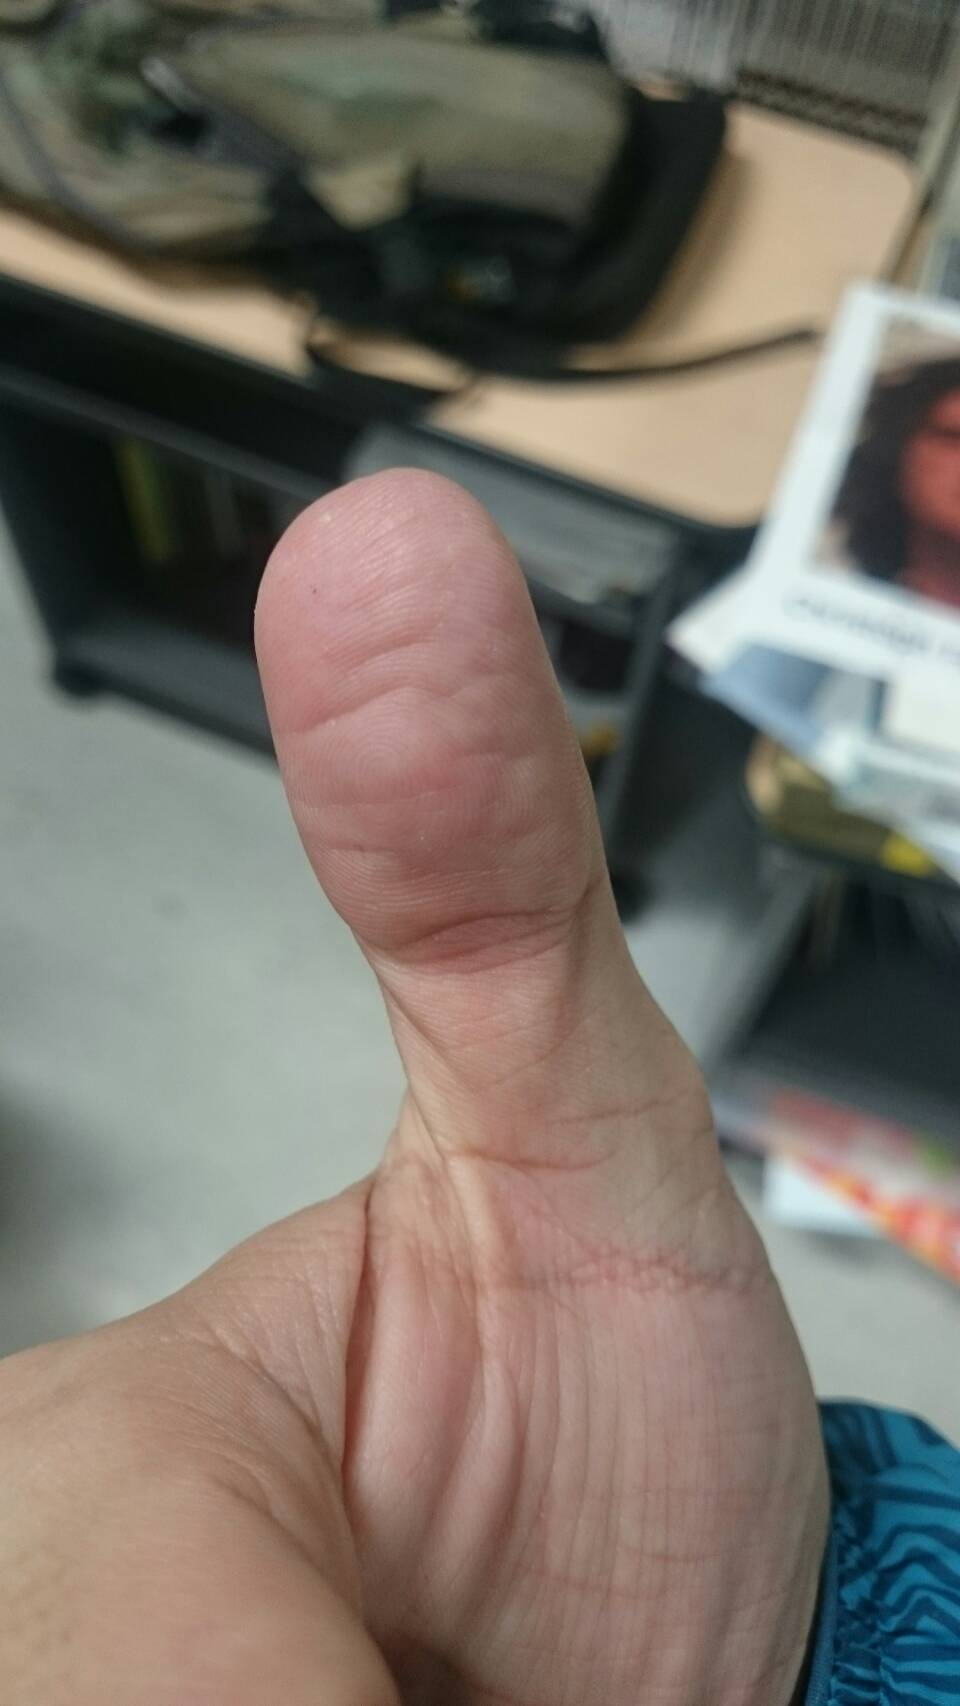
\includegraphics[scale=0.15]{takeda.jpg}
    \subcaption{タケダ氏}
  \end{minipage}
  \caption{各人の個人的な親指概要図}
 \end{figure}

さらに親指が変形し、豚指になってしまった新人種について示す。
この豚指については今後、学会等での発表など精力的な研究が行われることを期待されたい。
特に新しい発見はなく、なぜ指が豚になってしまったのか、なぜ長時間煮込んでもスープにならなかったのか、究明が急がれる。
\begin{figure}
\centering
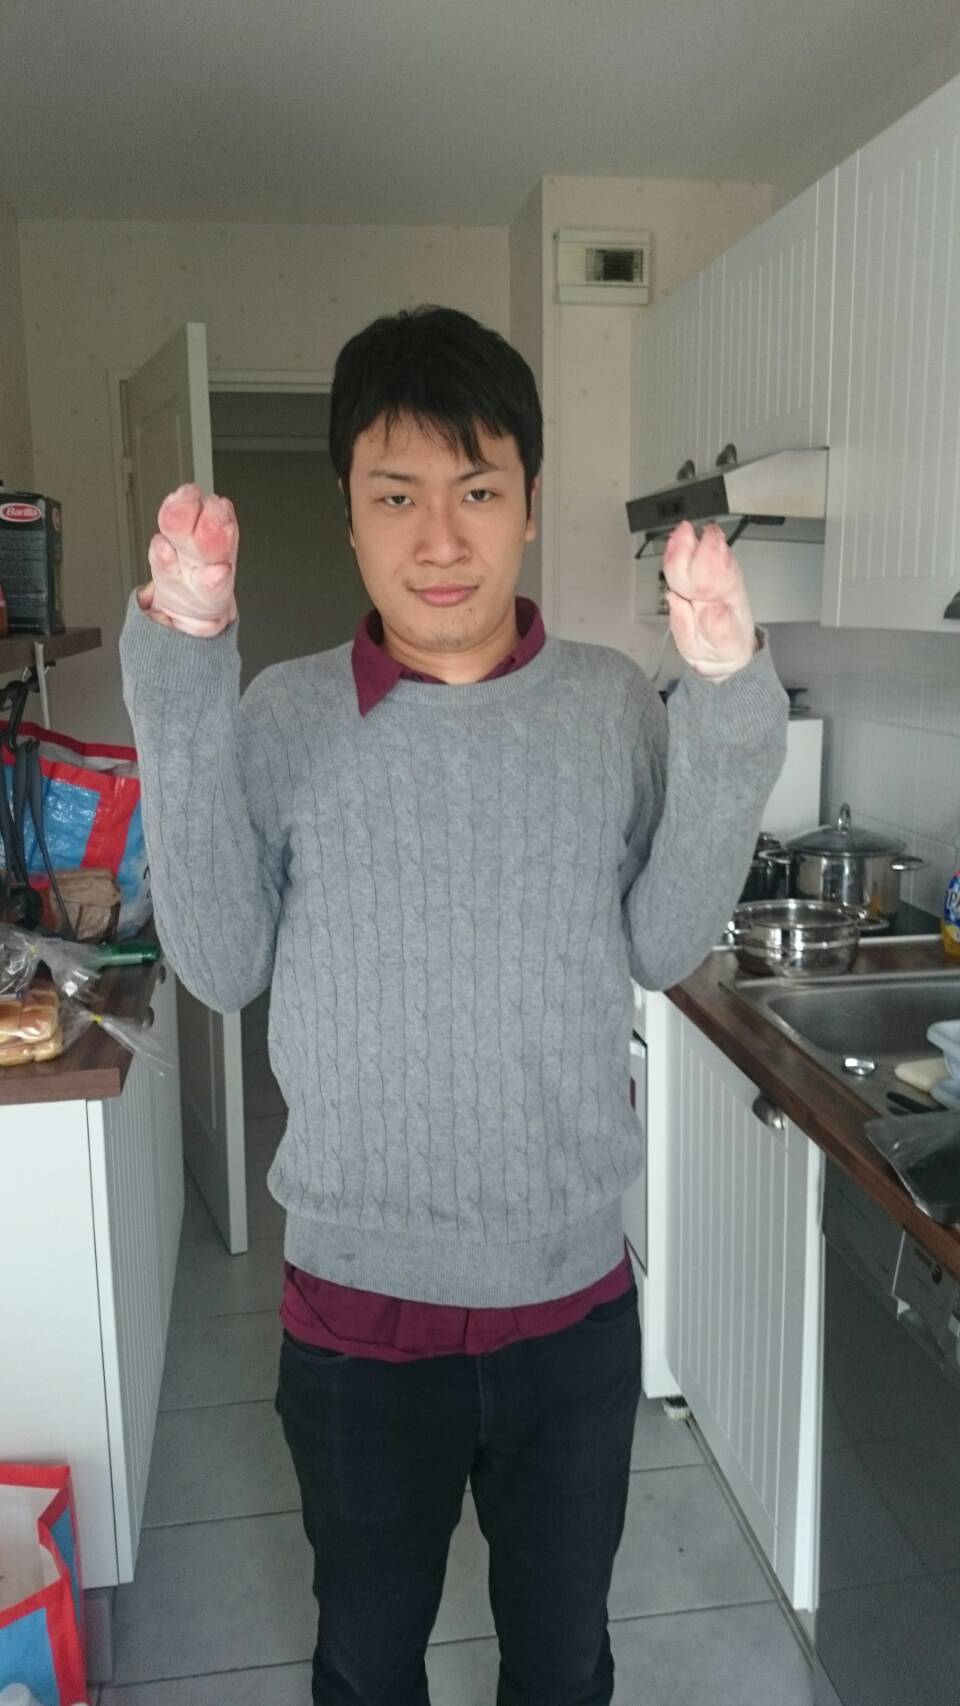
\includegraphics[scale=0.2]{ogawa.jpg}
\caption{豚指の概要図}
\end{figure}

\newpage
\clearpage
